\documentclass{article}
\usepackage{graphicx} % Required for inserting images
\usepackage{amsmath,amsfonts,amssymb,amsthm,mathtools}
\usepackage{relsize}
\usepackage{fullpage}
\usepackage{bigints}
\usepackage{float}
\usepackage{subfigure}
\usepackage{captcont}
\usepackage{lmodern} 			%accents and marks over letters
\usepackage[T1]{fontenc}		%accents and marks over letters
\usepackage{gensymb}
\usepackage{textcomp}
%\usepackage{lineno}		%add line numbers
\usepackage{color}
\usepackage{verbatim}
\usepackage{comment}
\usepackage{hyperref}		%make hyperlinks
\usepackage{array}
\usepackage{tabularx}
%\biboptions{square,numbers,sort&compress}
\graphicspath
{
{./figures/}
}

\title{Project 1: Bitcoin Price Prediction}
\author{Hoda Abokhadra\thanks{hoda2@illinois.edu},
Philip Myint\thanks{pcmyint2@illinois.edu}, 
Bryan Reynolds\thanks{bryanmr3@illinois.edu}, 
Taha Wasiq\thanks{twasiq2@illinois.edu}
\\CS 598: Practical Statistical Learning (Fall 2025)
\\University of Illinois Urbana-Champaign}
\date{\today}

\begin{document}

\maketitle

\section{Introduction}

Our goal in this project is to analyze and predict Bitcoin prices at two distinct time horizons, next day vs.\ next week, with the expectation that the latter will be more challenging to predict accurately. To achieve this purpose, we have cleaned a raw data file (e.g., by removing missing or invalid values) and produced many additional features based on common finance/banking industry metrics, selected and implemented regression models with varying degrees of sophistication, and applied those models to make price predictions and analyze/interpret our results. These are the subjects of Sections~\ref{sec:data_cleaning_configuration},~\ref{sec:methodology}, and~\ref{sec:results} of this report, respectively. We conclude in Section~\ref{sec:conclusions} with a brief summary of our findings. Our code is developed in \texttt{Python} and hosted on Github at \url{https://github.com/TahaWasiq/CS\_598\_Project\_1/}, with the following directory structure:
\begin{itemize}
    \item \textbf{\texttt{scripts\_cleaning/}}: Contains the data cleaning and configuration scripts described in Section~\ref{sec:data_cleaning_configuration}.
    \item \textbf{\texttt{data/}}: The raw, original csv Bitcoin prices data file and the various cleaned/reorganized data files.
    \item \textbf{\texttt{scripts\_models/}}: Scripts for analyzing the data, fitting the models, and performing model selection. Our modeling methodology is explained in Section~\ref{sec:methodology}, and the results are presented in Section~\ref{sec:results}.
    \item \textbf{\texttt{report/}}: Contains the figures and \LaTeX ~files used to generate this report.
\end{itemize}

\section{Data Cleaning and Configuration}
\label{sec:data_cleaning_configuration}

\subsection{Overview of pipeline}
We divide our data cleaning and configuration operations over five scripts that we run in the following order:

\begin{enumerate}
    \item \textbf{\texttt{clean.py}}: Takes the raw \textbf{bitcoin.csv} file and produces a cleaned version \textbf{bitcoin\_aligned.csv}.
    \item \textbf{\texttt{build-features.py}}: Reads \textbf{bitcoin\_aligned.csv} and produces dozens of additional features to produce two csv files: \textbf{btc\_features\_h1\_full.csv} and \textbf{btc\_features\_h7\_full.csv}, which may be used for predicting the Bitcoin price in the next day~(i.e., with a horizon of $h=1$ days) and the next week ($h=7$~days), respectively.
    \item \textbf{\texttt{split.py}}: Standardizes (produces $z$-scores) on the features in \textbf{btc\_features\_h1\_full.csv} and \textbf{btc\_features\_h7\_full.csv}, and breaks the data in each of these two files into training, validation, and test sets, for a total of six sets. Each set is stored in its own csv file.
    \item \textbf{\texttt{remove\_features\_vif.py}}: Calculates the variance inflation factor (VIF) for each feature and removes the ones that have a high VIF to improve the interpretability of the subsequent regression models.
    \item \textbf{\texttt{checks.py}}: Outputs summary statistics of the training, validation, and test sets, and verifies that none of the sets contain \texttt{NA} values.
\end{enumerate}

\noindent More details on each of these steps in our pipeline are described in the following subsections.

\subsection{Initial cleaning}
\textbf{\texttt{clean.py}} renames some of the columns in the raw \textbf{bitcoin.csv} file (e.g., \textbf{btc\_trade\_volume} is renamed to \textbf{btc\_volume}). Values in three critical columns (\textbf{btc\_close} [renamed from \textbf{btc\_market\_price}], \textbf{btc\_mktcap}, and \textbf{btc\_volume}) are converted/coerced to numeric values. \texttt{NA} values in these columns~are forward-filled by nearby non-\texttt{NA} ones. If there is a duplicate date, the second one is kept. Finally, a column for the \%~daily change is added, with all the aforementioned changes saved to a new file, \textbf{bitcoin\_aligned.csv}.

\subsection{Additional features}
Using \textbf{\texttt{build-features.py}}, we have created a large number of additional features (a total of 69), some of which are inspired by metrics commonly used in the finance/banking industries. These features include:
\begin{itemize}
    \item \textbf{btc\_rsi14}: The Relative Strength Index (RSI), a common finance metric used to measure momentum. Based on a rolling window of daily price changes averaged over the past 14 days, RSI captures recent buying vs.\ selling pressure (i.e., whether recent price changes have been mostly upward or downward).
    \item \textbf{btc\_ema12} and \textbf{btc\_ema26}: The average closing price over the last 12 days and 26 days, respectively, with more weight placed on recent days (an exponentially weighted moving average [EMA]).
    \item \textbf{btc\_macd}: Difference between a short-term trend (12-day EMA) and a longer-term trend (26-day EMA). If it’s positive, short-term momentum is stronger, if negative, momentum is weaker.
    \item \textbf{btc\_atr14}: The average size of daily price moves over the past 14 days, indicating price volatility.
\end{itemize}
In addition, the features include rolling means and standard deviations over the past 7, 14, and 30 days of the closing price, returns (\% change), and trading volume. We also include values of the closing price, returns, and volume from the previous day (1-day lag) and two weeks ago (15-day lag). Rows that have missing or invalid~(\texttt{NA}) values are dropped; this is the cleaning step where the first 5--6 months of data collected in 2010 were dropped, since the reported Bitcoin market price in the raw csv file remained flat at \$0 during that early period so that the \%~daily change and features based on that metric were undefined for those rows. As mentioned above, we save our additional features in two new files: \textbf{btc\_features\_h1\_full.csv} and \textbf{btc\_features\_h7\_full.csv}. The target columns in these files represent the Bitcoin price at the close of the next~day~($h=1$) and the next~week~($h=7$), respectively. Furthermore, these files contain a column for the date and a column for each of the 69~features, for a total of 71~columns in each file.

\subsection{Data splitting and standardization}
As its name implies, \textbf{\texttt{split.py}} splits \textbf{btc\_features\_h1\_full.csv} and \textbf{btc\_features\_h7\_full.csv} into training, validation, and test sets, producing a total of six new csv files (three for $h=1$ and another three for $h=7$). These sets are split chronologically, so that the first 70\% of entries are put into the training set, the next 15\% in the validation set, and the last 15\% in the test set. The idea is to develop models that can predict more recent trends after being trained on older trends. That is, we will train our models on historical data, tune/validate hyperparameters with more near-term data, and then finally test our models on the most recent data. Each of the 69 features are standardized so that they are transformed to $z$-scores based on means and standard deviations computed from the training set.

\subsection{Analyzing collinearity and removing high VIF features}
We check for collinearity by running a VIF analysis with \textbf{\texttt{remove\_features\_vif.py}}. The heart of this script is a function that recursively removes the feature with the highest VIF, until none of the remaining features have a VIF that lies above a specified threshold. By default, we set the threshold to a rather high value of~1000 so that only features that are strongly linearly correlated with at least one other feature are removed. This ends up removing 11 of our features so that we end up with a total of $69 - 11 = 58$. We could have chosen a more typical VIF threshold of 5 or 10, but our approach at this stage is to be cautious and avoid prematurely removing features that could end up being important. The regularization that we apply in Section~\ref{sec:methodology} provides another opportunity to remove highly collinear features in a more systematic manner.

\subsection{Data checks and verification}
The last step in our data cleaning and configuration pipeline is to run \textbf{\texttt{checks.py}}, which outputs summary statistics of the training, validation, and test sets, and verifies that none of the sets contain \texttt{NA} values. Table~\ref{tab:datasets} provides a summary of the final, cleaned version of our data sets. 

\begin{table}[ht]
\begin{center}
\caption{\label{tab:datasets} Number of days (i.e., number of rows in each file), start date, and end date for each of the six data sets after applying the cleaning and configuration operations described in Section~\ref{sec:data_cleaning_configuration}. Each file contains 58~features. For reference, the raw csv file contains 2920 rows spanning from 2010-02-23 to 2018-02-20, with 22 features. The vast majority of the $\sim$300 rows that were dropped are in the first several months of 2010, where the Bitcoin price is listed at \$0 in the raw file. Other reasons for dropping include duplicate dates or missing/invalid entries for the target or features.}
\begin{tabular}{| l | c c c|} 
 \hline
 \hspace{50pt}Data set & Number of days & Start date & End date \\ 
 \hline
 Next-day prediction ($h=1$) training set & 1877 & 2010-09-16 & 2015-12-07 \\ 
 Next-day prediction ($h=1$) validation set & 402 & 2015-12-08 & 2017-01-12 \\ 
 Next-day prediction ($h=1$) test set & 403 & 2017-01-13 & 2018-02-19 \\ 
 Next-week prediction ($h=7$) training set & 1873 & 2010-09-16 & 2015-12-03 \\
 Next-week prediction ($h=7$) validation set & 401 & 2015-12-04 & 2017-01-07 \\ 
 Next-week prediction ($h=7$) test set & 402 & 2017-01-08 & 2018-02-13 \\  
 \hline
\end{tabular}
\end{center}
\end{table}
\vspace{-20pt}
\section{Methodology}
\label{sec:methodology}

We apply the following four regression models to each of the $h = 1$ and~$h = 7$ data sets:
\begin{enumerate}
    \item Linear regression involving all of the~58~features without any regularization,
    \item Lasso regression,
    \item Ridge regression,
    \item Cubic B-Splines on four features combined together with ridge regression.
\end{enumerate}
These methods allow us to compare a naive approach (straightforward linear regression) with more sophisticated approaches that involve regularization and/or different basis functions (cubic polynomials in the case of the splines). For all the models, we determine the regression coefficients by fitting to the training data, and we select the best models for $h = 1$ and~$h = 7$ based on their performance on the corresponding validation set. We then analyze the performance of the chosen best models on the test set, focusing on mean-squared error~(MSE) and $R^2$~scores, as well as on model interpretation, as illustrated further in Section~\ref{sec:results}.

Our code is organized into a notebook, \textbf{\texttt{regression\_models.py}}, that interacts with users on the front~end and calls a utility file \textbf{\texttt{Utilities.py}} and a second script \textbf{\texttt{BitcoinModeler.py}} that does much of the work on the back~end by implementing the model initialization, fitting, evaluations, etc.\ in a series of classes (e.g., \textbf{\texttt{DataManager}}, \textbf{\texttt{ModelWrapper}}, \textbf{\texttt{ExperimentRunner}}). Data is read and manipulated in the form of \textbf{\texttt{Pandas DataFrames}} or \textbf{\texttt{NumPy}} arrays. We extensively utilize the \textbf{\texttt{sklearn}} package. In particular, we use the \textbf{\texttt{RidgeCV}} and \textbf{\texttt{LassoCV}} models in \textbf{\texttt{sklearn}}, with the regularization parameter~$\lambda$ selected through cross-validation over 500~logarithmically spaced values from $10^{-6}$ to $10^6$. We implement our spline model as a custom class that is based on the~\textbf{\texttt{SplineTransformer}} function in \textbf{\texttt{sklearn}}. The splines augment a linear ridge regressor with a small set of cubic B-spline basis functions to capture smooth, nonlinear effects while keeping the model regularized. From a hand-curated pool of potentially smooth signals (e.g., price, EMA/macd, RSI, rolling stats), we select at most~4 of these features to create B-spline basis functions that augment the ridge regressor. This feature selection is done using \textbf{\texttt{mutual\_info\_regression}} (MI), as defined in \textbf{\texttt{sklearn}}, that we compute on the training set only to avoid leakage. MI is preferred over Pearson correlation because it detects nonlinear and nonmonotonic dependencies between each candidate feature and the target, and it is invariant to monotone rescalings; this makes it a better filter for signals whose effect on the target is not strictly linear. For the chosen drivers, we expand them with \textbf{\texttt{SplineTransformer(degree=3, knots="quantile", extrapolation="linear")}}, concatenate the raw passthrough features, and fit a ridge penalty to control the increased degrees of freedom. Hyperparameters, like the number of knots and regularization parameter~$\lambda$, are tuned with a grid search. Limiting the number of spline features and using quantile-spaced knots keeps the basis compact, and it focuses capacity where the data are dense to reduce overfitting risk.

\section{Results}
\label{sec:results}

\begin{figure}[ht]
    \centering
    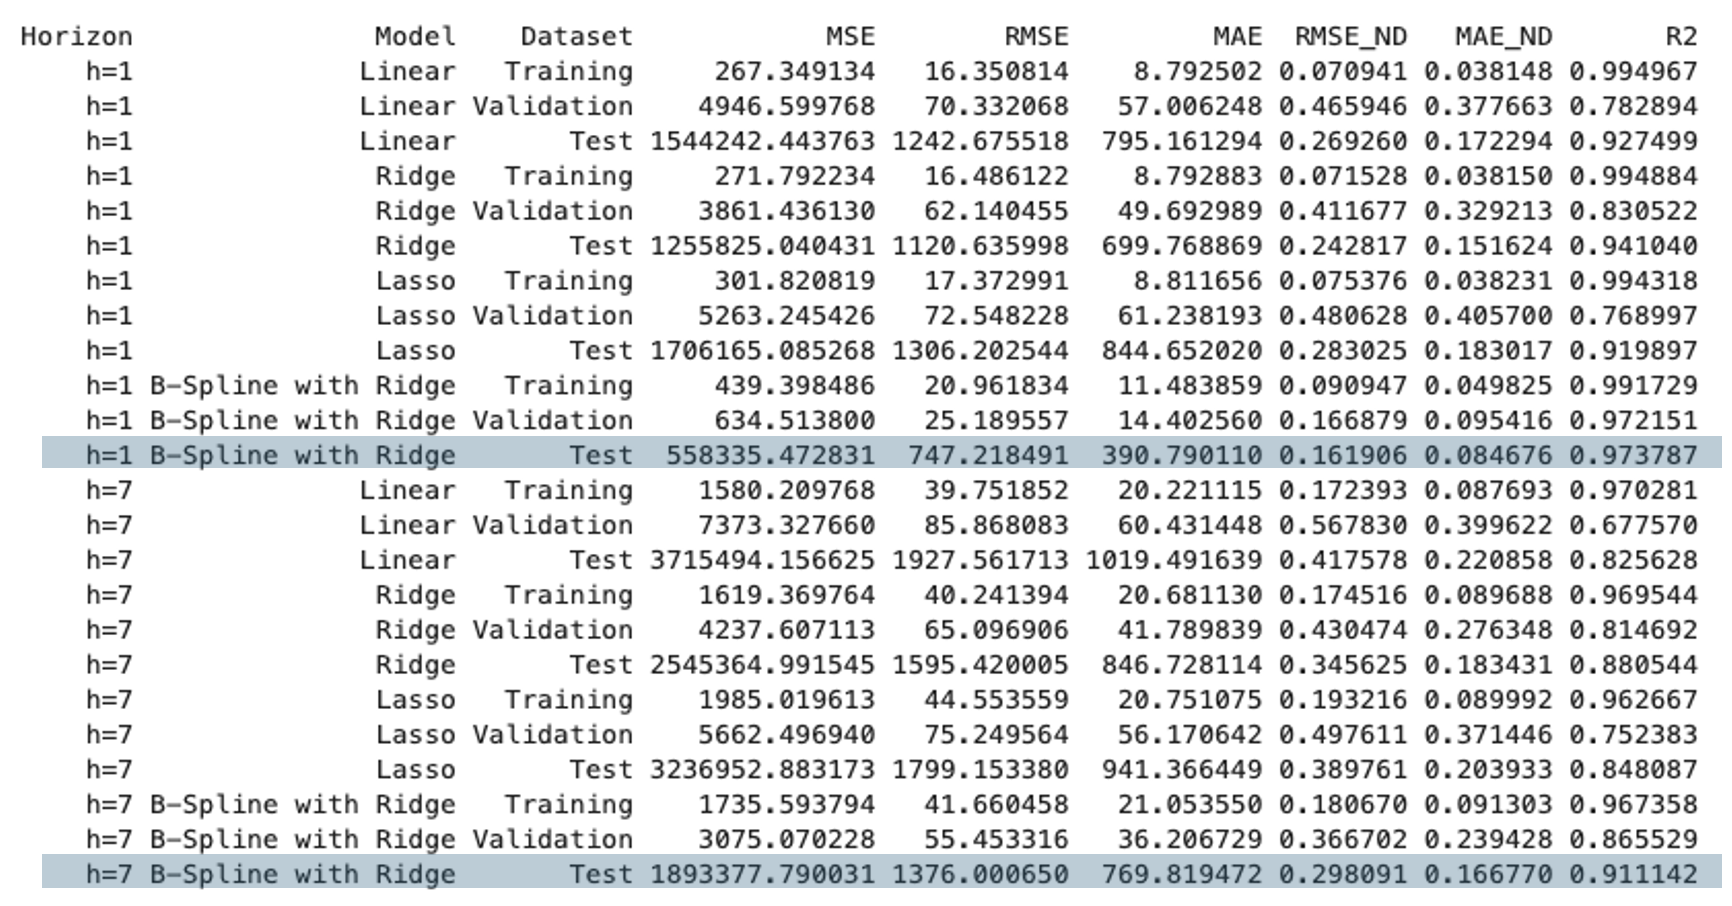
\includegraphics[width=0.95\linewidth]{figures/summary_table_highlight.png}
    \caption{Results for the four regression models on the two horizons. For both horizons, the model that performs best on the validation set and test set is the B-Spline with Ridge model, highlighted in blue. RMSE\_ND and MAE\_ND denote nondimensionalized versions of the root-mean-squared error (RMSE) and mean absolute error (MAE), respectively, which align well with trends in $R^2$, as explained in the text.}
    \label{fig:summary_table}
\end{figure}

The table in Figure~\ref{fig:summary_table} summarizes our results for all four regression models on the two horizons $h=1$ and $h=7$. For both horizons, the B-spline with Ridge model performs best on all metrics for the validation set, meaning it has the lowest MSE, lowest mean absolute error (MAE), and highest~$R^2$ on the validation set. As a result, we designate it as our best model, and from the table, we see that it also has the best performance on the test set as well. Interestingly, the other models tend to perform better on the training set, but worse on the validation and training sets, which is a manifestation of the bias--variance tradeoff. This suggests that the B-spline with Ridge model is relatively robust to variances that stem from the validation and test sets being taken from later dates (see~Table~\ref{tab:datasets}), variances that reflect increases in the Bitcoin price over time. In particular, the test set exhibits a dramatic increase in the price, as seen in Figure~\ref{fig:prices_h1}. The MSE and MAE are orders of magnitude higher in the test set than in the validation set, despite the models generally having a higher $R^2$ score on the test set, simply because the average price and variance in the test set is much higher. To account for this, we have produced nondimensionalized versions of RMSE and MAE where we divide these quantities by the standard deviations of the true target values. The table in Figure~\ref{fig:summary_table} shows that the nondimensionalized RMSE and MAE follow the same trends as $R^2$ on the test set vs.\ the validation set. 

\begin{figure}
    \centering
    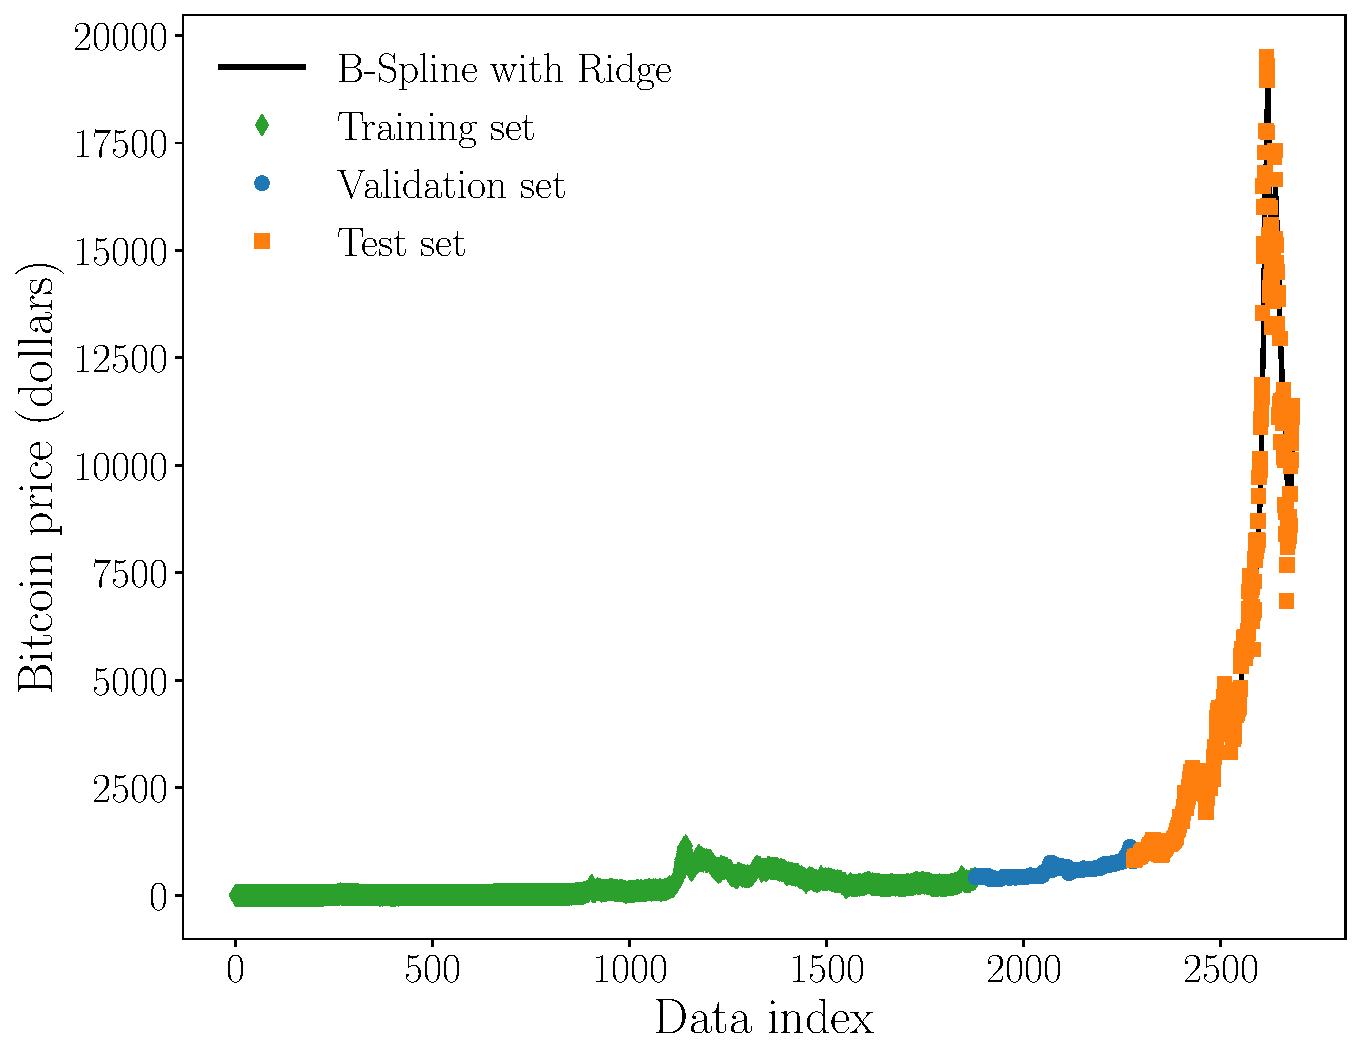
\includegraphics[width=0.45\linewidth]{figures/bitcoin_prices_h1.pdf}
    \caption{Time series of Bitcoin prices. The $x$-axis denotes the data index (row index), which is a surrogate for the date because the files are sorted chronologically. Results here are for~$h=1$ (plot for $h=7$ is similar).}
    \label{fig:prices_h1}
\end{figure}

\begin{figure}[ht]
    \centering
    (a)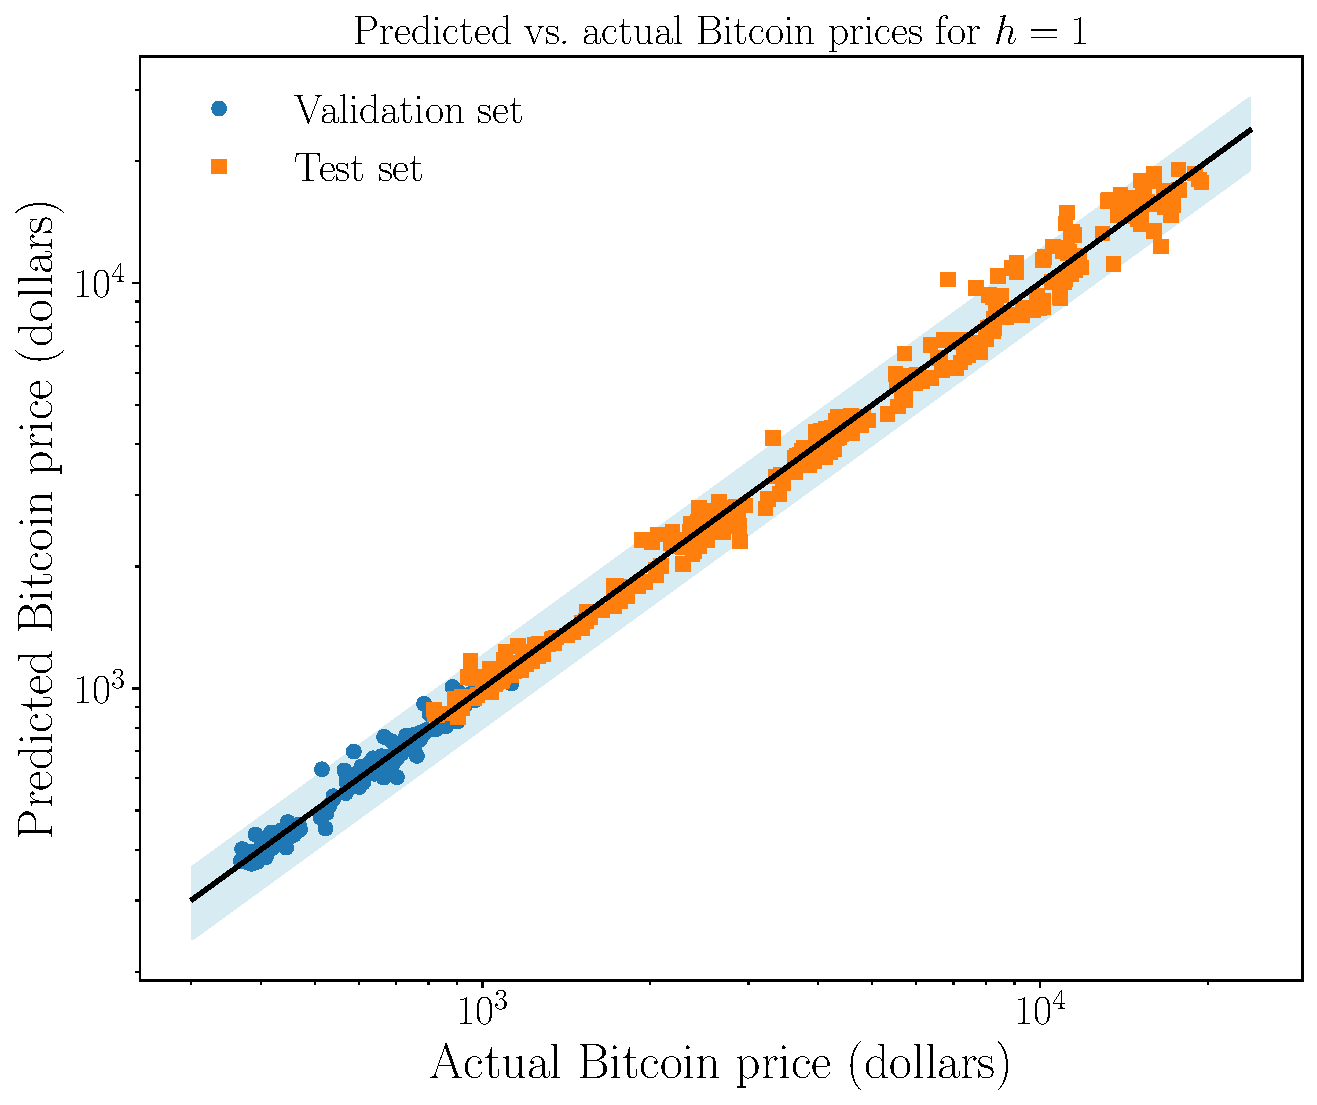
\includegraphics[width=0.45\linewidth]{figures/actual_vs_predicted_h1.pdf}
    (b)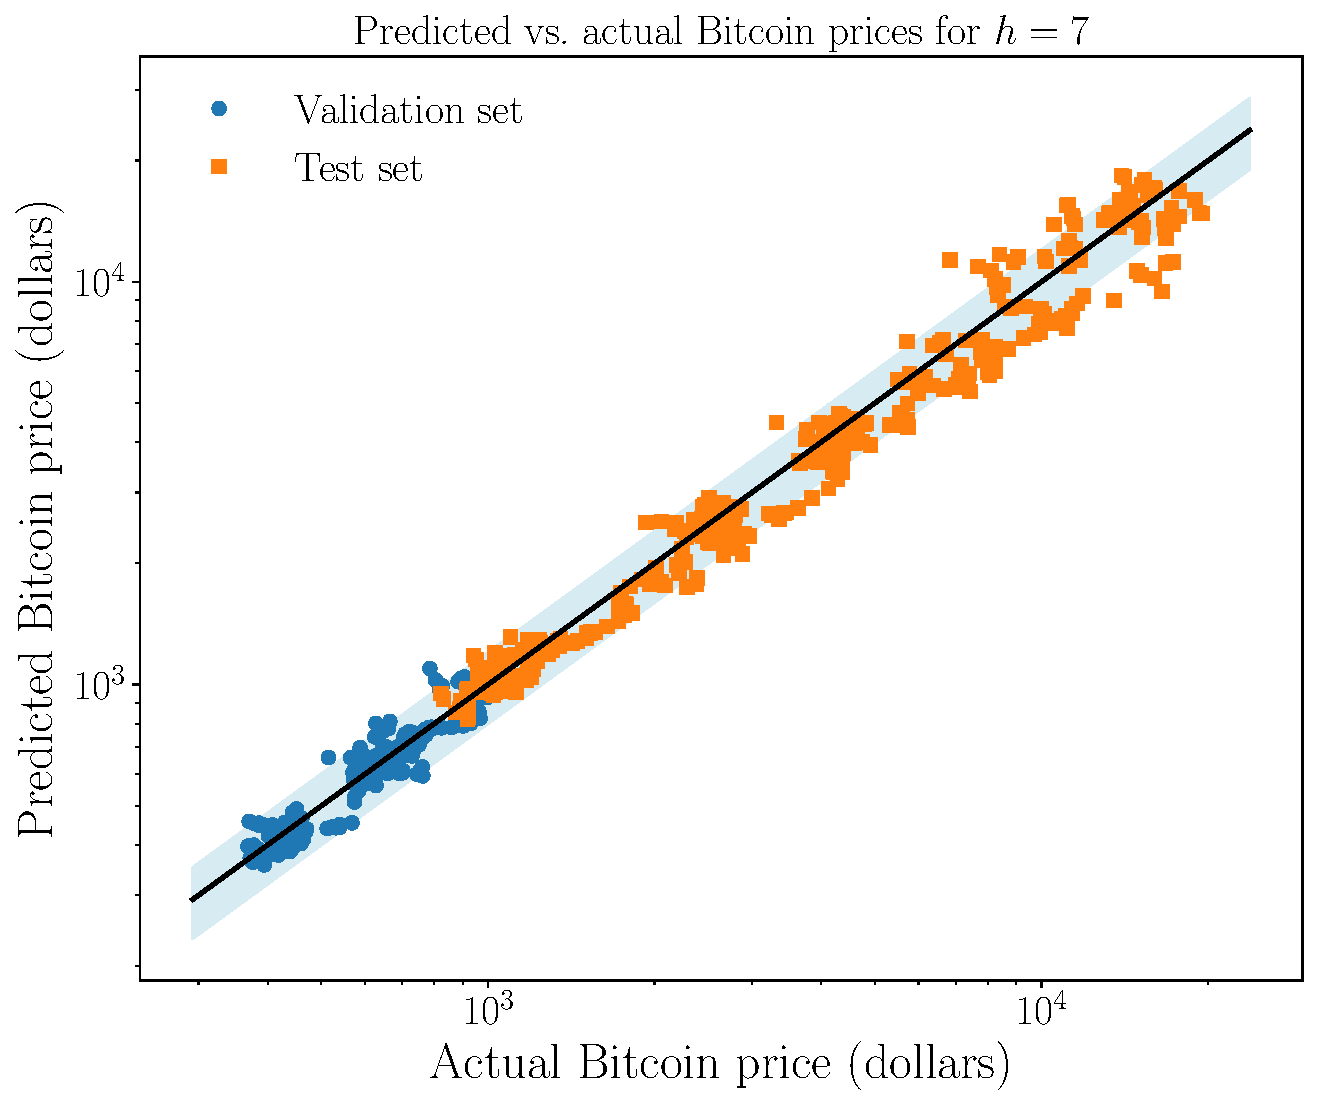
\includegraphics[width=0.45\linewidth]{figures/actual_vs_predicted_h7.pdf}
    \caption{Predicted vs.\ actual Bitcoin prices for the B-spline with Ridge model for:~(a)~the $h=1$ horizon and~(b)~the $h=7$ horizon. The black line shows the line $y=x$, indicating a perfect prediction, and the blue band denotes $\pm$20\% error bars around that line.}
    \label{fig:actual_vs_predicted}
\end{figure}

\begin{figure}[ht]
    \centering
    (a)
\includegraphics[width=0.45\linewidth]{figures/h1_lasso_coefs.pdf}
    (b)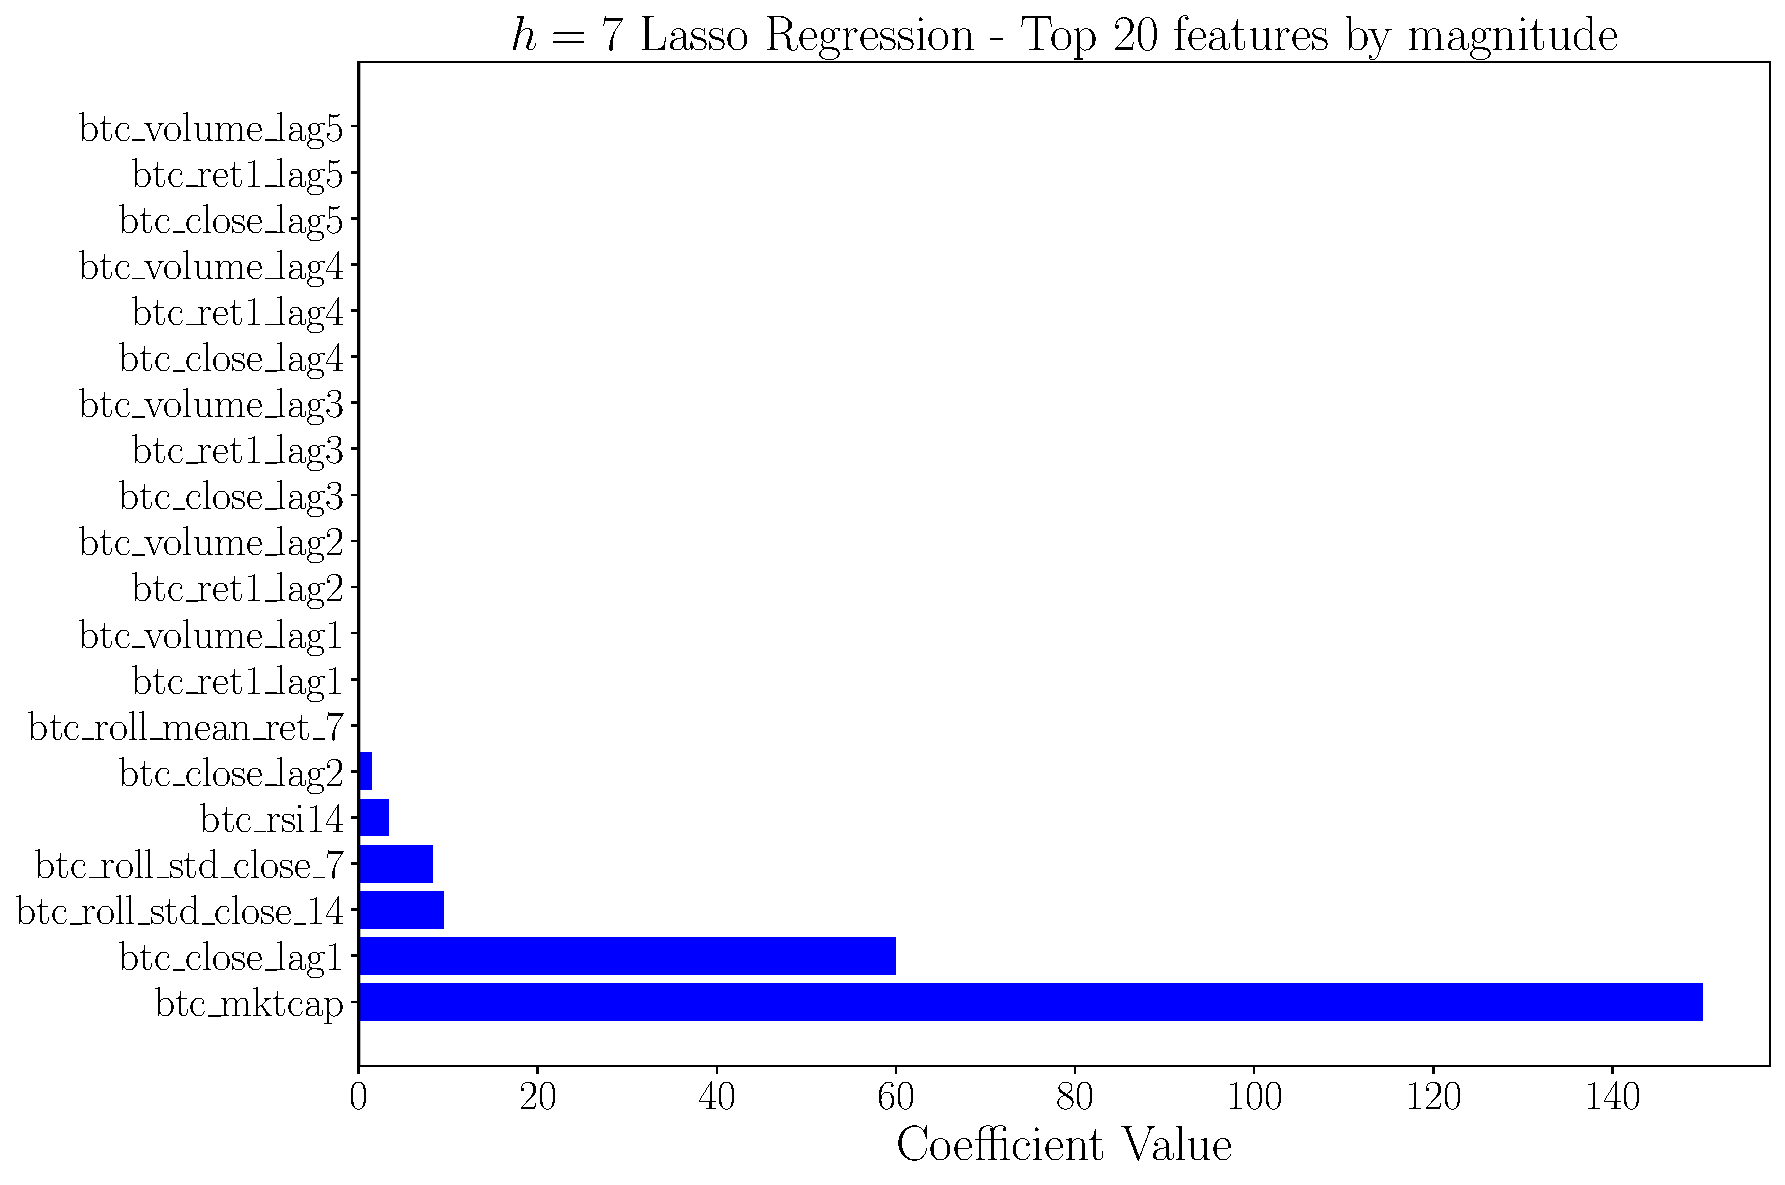
\includegraphics[width=0.45\linewidth]{figures/h7_lasso_coefs.pdf}
    \caption{Top~20 regression coefficients by magnitude for the Lasso model for~a)~$h=1$ and~(b)~$h=7$.}
    \label{fig:lasso_coefficients}
\end{figure}

Another trend that we observe from the summary table is that all the models perform better for the $h=1$ horizon than the $h=7$ horizon. Figure~\ref{fig:actual_vs_predicted} illustrates this for the particular example of the B-spline with Ridge model. For~$h=1$, the model is able to predict nearly all of the data points to within an error of~$\pm$20\%, whereas for~$h=7$, there are noticeably more points that fall outside of that error band. This agrees with the intuitive notion that the task of predicting the price in the next day ($h=1$) would be easier than predicting a more distant price in the future, such as next week~($h=7$). Inspection of the model coefficients reveals more insight into the differences between the two time horizons. Out of the 58 features, Lasso shrinks all but 20 of them to zero for~$h=1$, and it goes even further for~$h=7$, where only 7 features have nonzero coefficients~(Figure~\ref{fig:lasso_coefficients}). This suggests that for predicting prices over longer time horizons, most of the features become irrelevant and only a small portion of them explain the observed variability. Interestingly, although there are fewer nonzero coefficients, the 2-norm of the coefficients vector is larger in~$h=7$, so there is a relatively heavy concentration in a smaller set of coefficients with elevated importance. Similar behavior (not shown in Figure~\ref{fig:lasso_coefficients} for brevity) is seen for the Ridge and B-Spline with Ridge models as well, although these models do not shrink any of the coefficients to zero. The Linear model unsurprisingly has the largest 2-norm, and it performs the worst on the validation and test sets for the~$h=7$ horizon precisely because it lacks the regularization needed to help concentrate the values in a smaller, but important subset of the~coefficients.

\section{Conclusions}
\label{sec:conclusions}

In summary, we have produced data files and scripts to analyze and make predictions on Bitcoin prices over two time horizons: $h=1$ (next day) and $h=7$ (next week). To prepare the data, we have added dozens of features, many of which are inspired from finance/banking, performed cleaning to remove invalid (\texttt{NA}) or missing values, and subsequently removed some of the features that have a very high~VIF to improve the model interpretability. The data for each horizon is split chronologically into training (first 70\%), validation (next 15\%), and test (last 15\%) sets, with each file containing 58~features that are standardized with data from the training set. We have applied four models to predict Bitcoin prices:~1)~linear regression without any regularization,~2)~lasso regression,~3)~ridge regression, and~4)~B-splines augmenting a ridge regressor. For both horizons, we find that the B-Spline with Ridge model performs best on the validation and test sets in terms of metrics like~$R^2$ and MSE, even if other models perform better on the training set, reflecting the bias--variance tradeoff. The B-Spline with Ridge model is relatively robust to variances in the data, including being able to handle the sharp rise and fall in Bitcoin prices that are exhibited in the test set but not present in the training set. It has an~$R^2$ score of about~0.97 and~0.91 on the $h=1$ and~$h=7$ test sets, respectively. In fact, all the models perform better on~$h=1$ than on~$h=7$, agreeing with the expectation that next-day prices should be easier to predict than prices in the next week. Inspection of the model coefficients reveals that the variability in the $h=7$ horizon is explained by a smaller subset of the features than in $h=1$, which suggests that more of the features become irrelevant as we attempt to predict prices further out in the future. This also underlines the importance of regularization (particularly for $h=7$), since it helps to temper the less important features. To further build on this report, one may explore other time horizons (perhaps 1~month) and other models introduced later in the class (e.g., random forests, support vector machines).

\end{document}
